\section{Flow Nets}
\textbf{Example 3: 2D Stream Function using Jacobi Iteration}
In steady aquifer flow, the flow is irrotational (or at least can be modeled as such). 
There exists an orthogonal function called the stream function (it is the function that exists in the flow field when vorticity is zero).
A really good explaination of stream functions (and streamlines) appears on pages 381--398 in \cite{Zheng1995}.

This function can be used to generate plots of streamlines for the same system.
The principal changes are the material properties representation and the boundary conditions.  

The stream function $\Psi$ as a partial differential equation is
\begin{equation}
0= 
\frac{\partial}{\partial x}({\frac{1}{T_y} \frac{\partial \Psi}{\partial x}})
+
\frac{\partial}{\partial y}({\frac{1}{T_x} \frac{\partial \Psi}{\partial y}})
\end{equation}

Observe how the material property is inverted and changes directional identity, otherwise the equation is structurally identical to the groundwater flow equation (for steady flow).

The difference equation is also almost the same

\begin{equation}
\begin{matrix}
0= 
[\frac{1}{\Delta x} \frac{1}{T_{y}} \frac{\Psi_{i-1,j} - \Psi_{i,j}}{\Delta x} +
 \frac{1}{\Delta y} \frac{1}{T_{x}} \frac{\Psi_{i,j-1} - \Psi_{i,j}}{\Delta y}] - \\
~~~~~~~~~~\\
~~~~~~~~~~[ \frac{1}{\Delta x} \frac{1}{T_{y}}  \frac{\Psi_{i,j} - \Psi_{i+1,j}}{\Delta x} +
  \frac{1}{\Delta y}  \frac{1}{T_{x}} \frac{\Psi_{i,j} - \Psi_{i,j+1}}{\Delta y} ]        
\end{matrix}        
\end{equation}

The substitutions are

\begin{equation}
\begin{matrix}
A_{i,j} = \frac{1}{2 \Delta x^2}(T_{y,(i-1,j)}^{-1}+T_{y,(i,j)}^{-1}) \\ ~~ \\
B_{i,j} = \frac{1}{2 \Delta x^2}(T_{y,(i,j)}^{-1}+T_{y,(i+1,j)}^{-1})   \\ ~~ \\
C_{i,j} = \frac{1}{2 \Delta y^2}(T_{x,(i,j-1)}^{-1}+T_{x,(i,j)}^{-1})   \\ ~~ \\
D_{i,j} = \frac{1}{2 \Delta y^2}(T_{x,(i,j)}^{-1}+T_{x,(i,j+1)}^{-1})   \\ ~~ \\
\end{matrix}
\end{equation}

Substitution into the difference equation yields

\begin{equation}
0 = A_{i,j}\Psi_{i-1,j} + B_{i,j}\Psi_{i+1,j} - (A_{i,j}+B_{i,j}+C_{i,j}+D_{i,j})\Psi_{i,j} + C_{i,j}\Psi_{i,j-1} + D_{i,j}\Psi_{i,j+1}
\end{equation}

As before we can explicitly write the cell equation for $h_{i,j}$ as

\begin{equation}
\Psi_{i,j} = \frac{[A_{i,j}\Psi_{i-1,j} + B_{i,j}\Psi_{i+1,j} + C_{i,j}\Psi_{i,j-1} + D_{i,j}\Psi_{i,j+1}]}{[A_{i,j}+B_{i,j}+C_{i,j}+D_{i,j}]}
\end{equation}

So at this point we could literally use the same script, however boundary conditions also ``invert.''
A no-flow head-domain boundary is a constant value stream function-domain boundary.
A constant value head-domain boundary is a zero-gradient stream function-domain boundary.

So we could use the same code, but probably are better off building a separate code (it can read the same input file), and use it to generate stream functions.  
The prior example code is modified to generate the stream function for its case (and plot the stream function contours), which if overlaid on the head contours produces a flow net.
%After the example is presented, the two contour plots will be overlaid outside of \textbf{R}.\footnote{I will be using macOS programs to render the two plots into a single plot.  
%What the analyst has to do is to make both plots and save them.  Then choose one plot, and render all ``white pixels" as transparent.  Then take this new image and import onto the other plot.  The result is a flownet for the aquifer system.} 

The modified code literally changes the names of the head array to stream function, modifies how the material properties ($A,B,C,D$) are constructed, and modified how the boundary conditions are incorporated.  Listing \ref{lst:2D-JacobiStream} is a listing that implements the method -- notice how the no-flow boundary conditions are implemented.   

In this example the value of the stream function is arbitrarily set to range from $0$ to $100$.  One useful interpretation of stream function values is that their differences indicate the flow fraction (of total flow) that flows between the streamlines (contour lines of constant stream function value).
\clearpage

\begin{lstlisting}[caption= R code demonstrating an Stream Function Simulator for 2D Steady Flow.  This code fragment implements the Jacobi iteration.  A subsequent listing shows the contour plot syntax.  In the example the two fragments are joined and run as a single source file \\ , label=lst:2D-JacobiStream]
# 2D-streamfunction
# Implements Finite-Difference Stream Function using Jacobi Iteration
# Assumes no-flow boundary row=1,and nrows ==> constant stream function
# Assumes fixed head boundary col=1, and ncols ==> no-flux stream function -- stream function runs from 0 to 100
zz <- file("input1.dat", "r") # Open a connection named zz to file named input.dat
# read the simulation conditons
deltax <-as.numeric(readLines(zz, n = 1, ok = TRUE, warn = TRUE,encoding = "unknown", skipNul = FALSE))
deltay <-as.numeric(readLines(zz, n = 1, ok = TRUE, warn = TRUE,encoding = "unknown", skipNul = FALSE))
deltaz <-as.numeric(readLines(zz, n = 1, ok = TRUE, warn = TRUE,encoding = "unknown", skipNul = FALSE))
nrows <-as.numeric(readLines(zz, n = 1, ok = TRUE, warn = TRUE,encoding = "unknown", skipNul = FALSE))
ncols <-as.numeric(readLines(zz, n = 1, ok = TRUE, warn = TRUE,encoding = "unknown", skipNul = FALSE))
tolerance <- as.numeric(readLines(zz, n = 1, ok = TRUE, warn = TRUE,encoding = "unknown", skipNul = FALSE))
streamfn <-(readLines(zz, n = nrows, ok = TRUE, warn = TRUE,encoding = "unknown", skipNul = FALSE))
hydcondx <-(readLines(zz, n = nrows, ok = TRUE, warn = TRUE,encoding = "unknown", skipNul = FALSE))
hydcondy <-(readLines(zz, n = nrows, ok = TRUE, warn = TRUE,encoding = "unknown", skipNul = FALSE))
close(zz)
# split the multiple column strings into numeric components for a vector
streamfn <-as.numeric(unlist(strsplit(streamfn,split=" ")))
hydcondx <-as.numeric(unlist(strsplit(hydcondx,split=" ")))
hydcondy <-as.numeric(unlist(strsplit(hydcondy,split=" ")))
# convert the numeric vectors into matrices for easier indexing
streamfn <-matrix(streamfn,nrow=nrows,ncol=ncols,byrow = TRUE)
hydcondx <-matrix(hydcondx,nrow=nrows,ncol=ncols,byrow = TRUE)
hydcondy <-matrix(hydcondy,nrow=nrows,ncol=ncols,byrow = TRUE)
# built the transmissivity arrays
amat<-matrix(0,nrows,ncols) 
bmat<-matrix(0,nrows,ncols) 
cmat<-matrix(0,nrows,ncols)
dmat<-matrix(0,nrows,ncols)
for(irow in 2:(nrows-1)){
  for(jcol in 2:(ncols-1)){
    amat[irow,jcol]<-((1.0/hydcondy[irow-1,jcol  ]+1.0/hydcondy[irow  ,jcol  ])*deltaz)/(2.0*deltax^2)
    bmat[irow,jcol]<-((1.0/hydcondy[irow  ,jcol  ]+1.0/hydcondy[irow+1,jcol  ])*deltaz)/(2.0*deltax^2)
    cmat[irow,jcol]<-((1.0/hydcondx[irow  ,jcol-1]+1.0/hydcondx[irow  ,jcol  ])*deltaz)/(2.0*deltay^2)
    dmat[irow,jcol]<-((1.0/hydcondx[irow  ,jcol  ]+1.0/hydcondx[irow  ,jcol+1])*deltaz)/(2.0*deltay^2)
  }
}
# begin the calculations
streamold<-streamfn # copy the head array, used to test for stopping 
maxit <- 100 # set the maximum number of iterations (to prevent infinite loop)
for (iter in 1:maxit){
  # first and last row special == no flow boundaries in head, fixed value streamfunction
  for(jcol in 1:ncols){
    streamfn[1,jcol]=0.0
    streamfn[nrows,jcol]=100.0
  }
  for (irow in 2:(nrows-1)){
  # first and last columns special == fixed head boundaries, no-gradient stream function
    streamfn[irow,1]=streamfn[irow,2]
    streamfn[irow,nrows]=streamfn[irow,nrows-1]
    for (jcol in 2:(nrows-1)){
      streamfn[irow,jcol] = 
        (amat[irow,jcol]*streamfn[irow-1,jcol  ] +
         bmat[irow,jcol]*streamfn[irow+1,jcol  ] +
         cmat[irow,jcol]*streamfn[irow  ,jcol-1] +
         dmat[irow,jcol]*streamfn[irow  ,jcol+1]  )/
        (amat[irow,jcol]+bmat[irow,jcol]+cmat[irow,jcol]+dmat[irow,jcol])
    }
  }
# test for stopping iterations
  percentdiff <- sum((streamfn-streamold)^2)
  if (percentdiff < tolerance){
    message("Exit iterations because tolerance met")
    break}
  streamold<-streamfn  #update the current head vector
}
}\end{lstlisting}
\clearpage

\begin{lstlisting}[caption= R code demonstrating an Stream Function Simulator for 2D Steady Flow.  This code fragment implements the contour plotting \\ , label=lst:2D-ContourStream]
# echo contents for debugging
# streamfn
# streamold
##############################################################
###    built position arrays for contour plotting          ###
##############################################################
distancex<-numeric(nrows)
distancey<-numeric(ncols)
distancex[1]<-50
distancey[1]<-50
for (irow in 2:nrows){distancex[irow]<-distancex[irow-1]+deltax}
for (jcol in 2:ncols){distancey[jcol]<-distancey[jcol-1]+deltay}
##############################################################
###    contour plot of head -- note axes are rotated       ###
##############################################################
contour(distancex,distancey,streamfn,
        plot.title = title(main = "Stream Function Model",
                           xlab = "Meters (Y axis) ====>>", 
                           ylab = "Meters (X axis) ====>>"))
}\end{lstlisting}

Figure \ref{fig:streamfn-2d-contour1} is the stream function result.  
Compare it to Figure \ref{fig:aquifer-2d-contour1} and it should be clear that the ``lines'' are at right angles to each other --that is the stream function is orthogonal to the head function (which is anticipated, because of the nature of the relationship between stream function and head functions; the orthogonality is a consequence of the flow satisfying the the Cauchy-Riemann conditions.).

\begin{figure}[h!] %  figure placement: here, top, bottom, or page
   \centering
   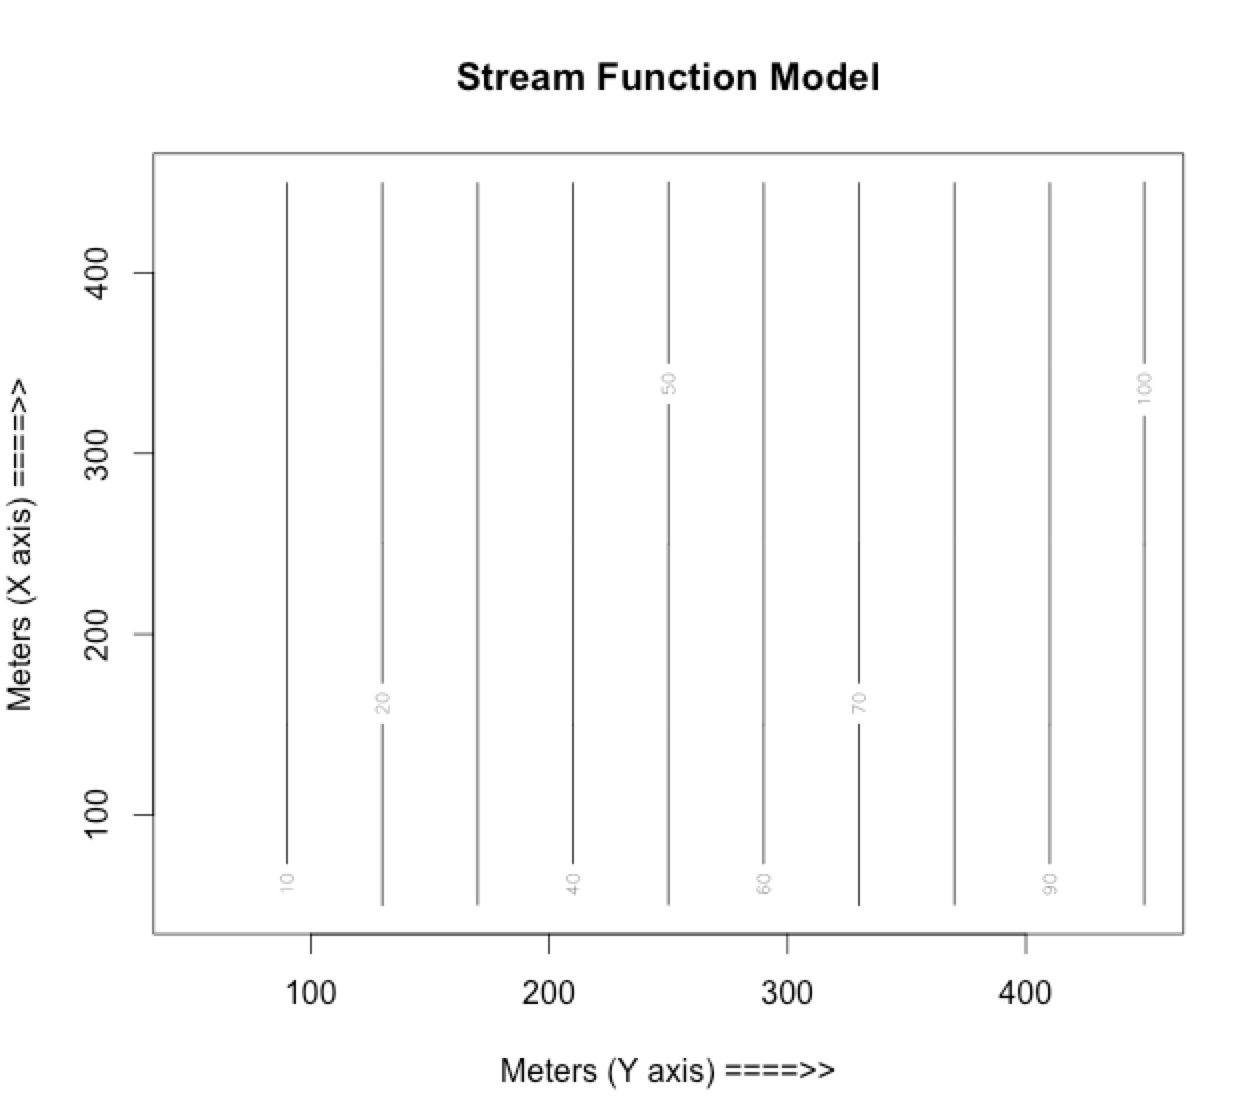
\includegraphics[height=4in]{./19-FlowNets/streamfn-2d-contour1.jpg} 
   \caption{Output from \textbf{R} script for stream function model.}
   \label{fig:streamfn-2d-contour1}
\end{figure}

To complete the example, and prepare for the next example, we will modify the script one more time to:
\begin{enumerate}
\item Read in the material property values, head values, etc.  (no change).
\item Compute the head distribution.
\item Compute the stream function distribution. (merge the two scripts)
\item Plot the head and stream function on the same graph -- use different colors.  Also rotate the plots so axes agree with the problem statement.
\end{enumerate}

Figure \ref{fig:streamfn-2d-contour2} is the result of these modifications.  


\begin{figure}[h!] %  figure placement: here, top, bottom, or page
   \centering
   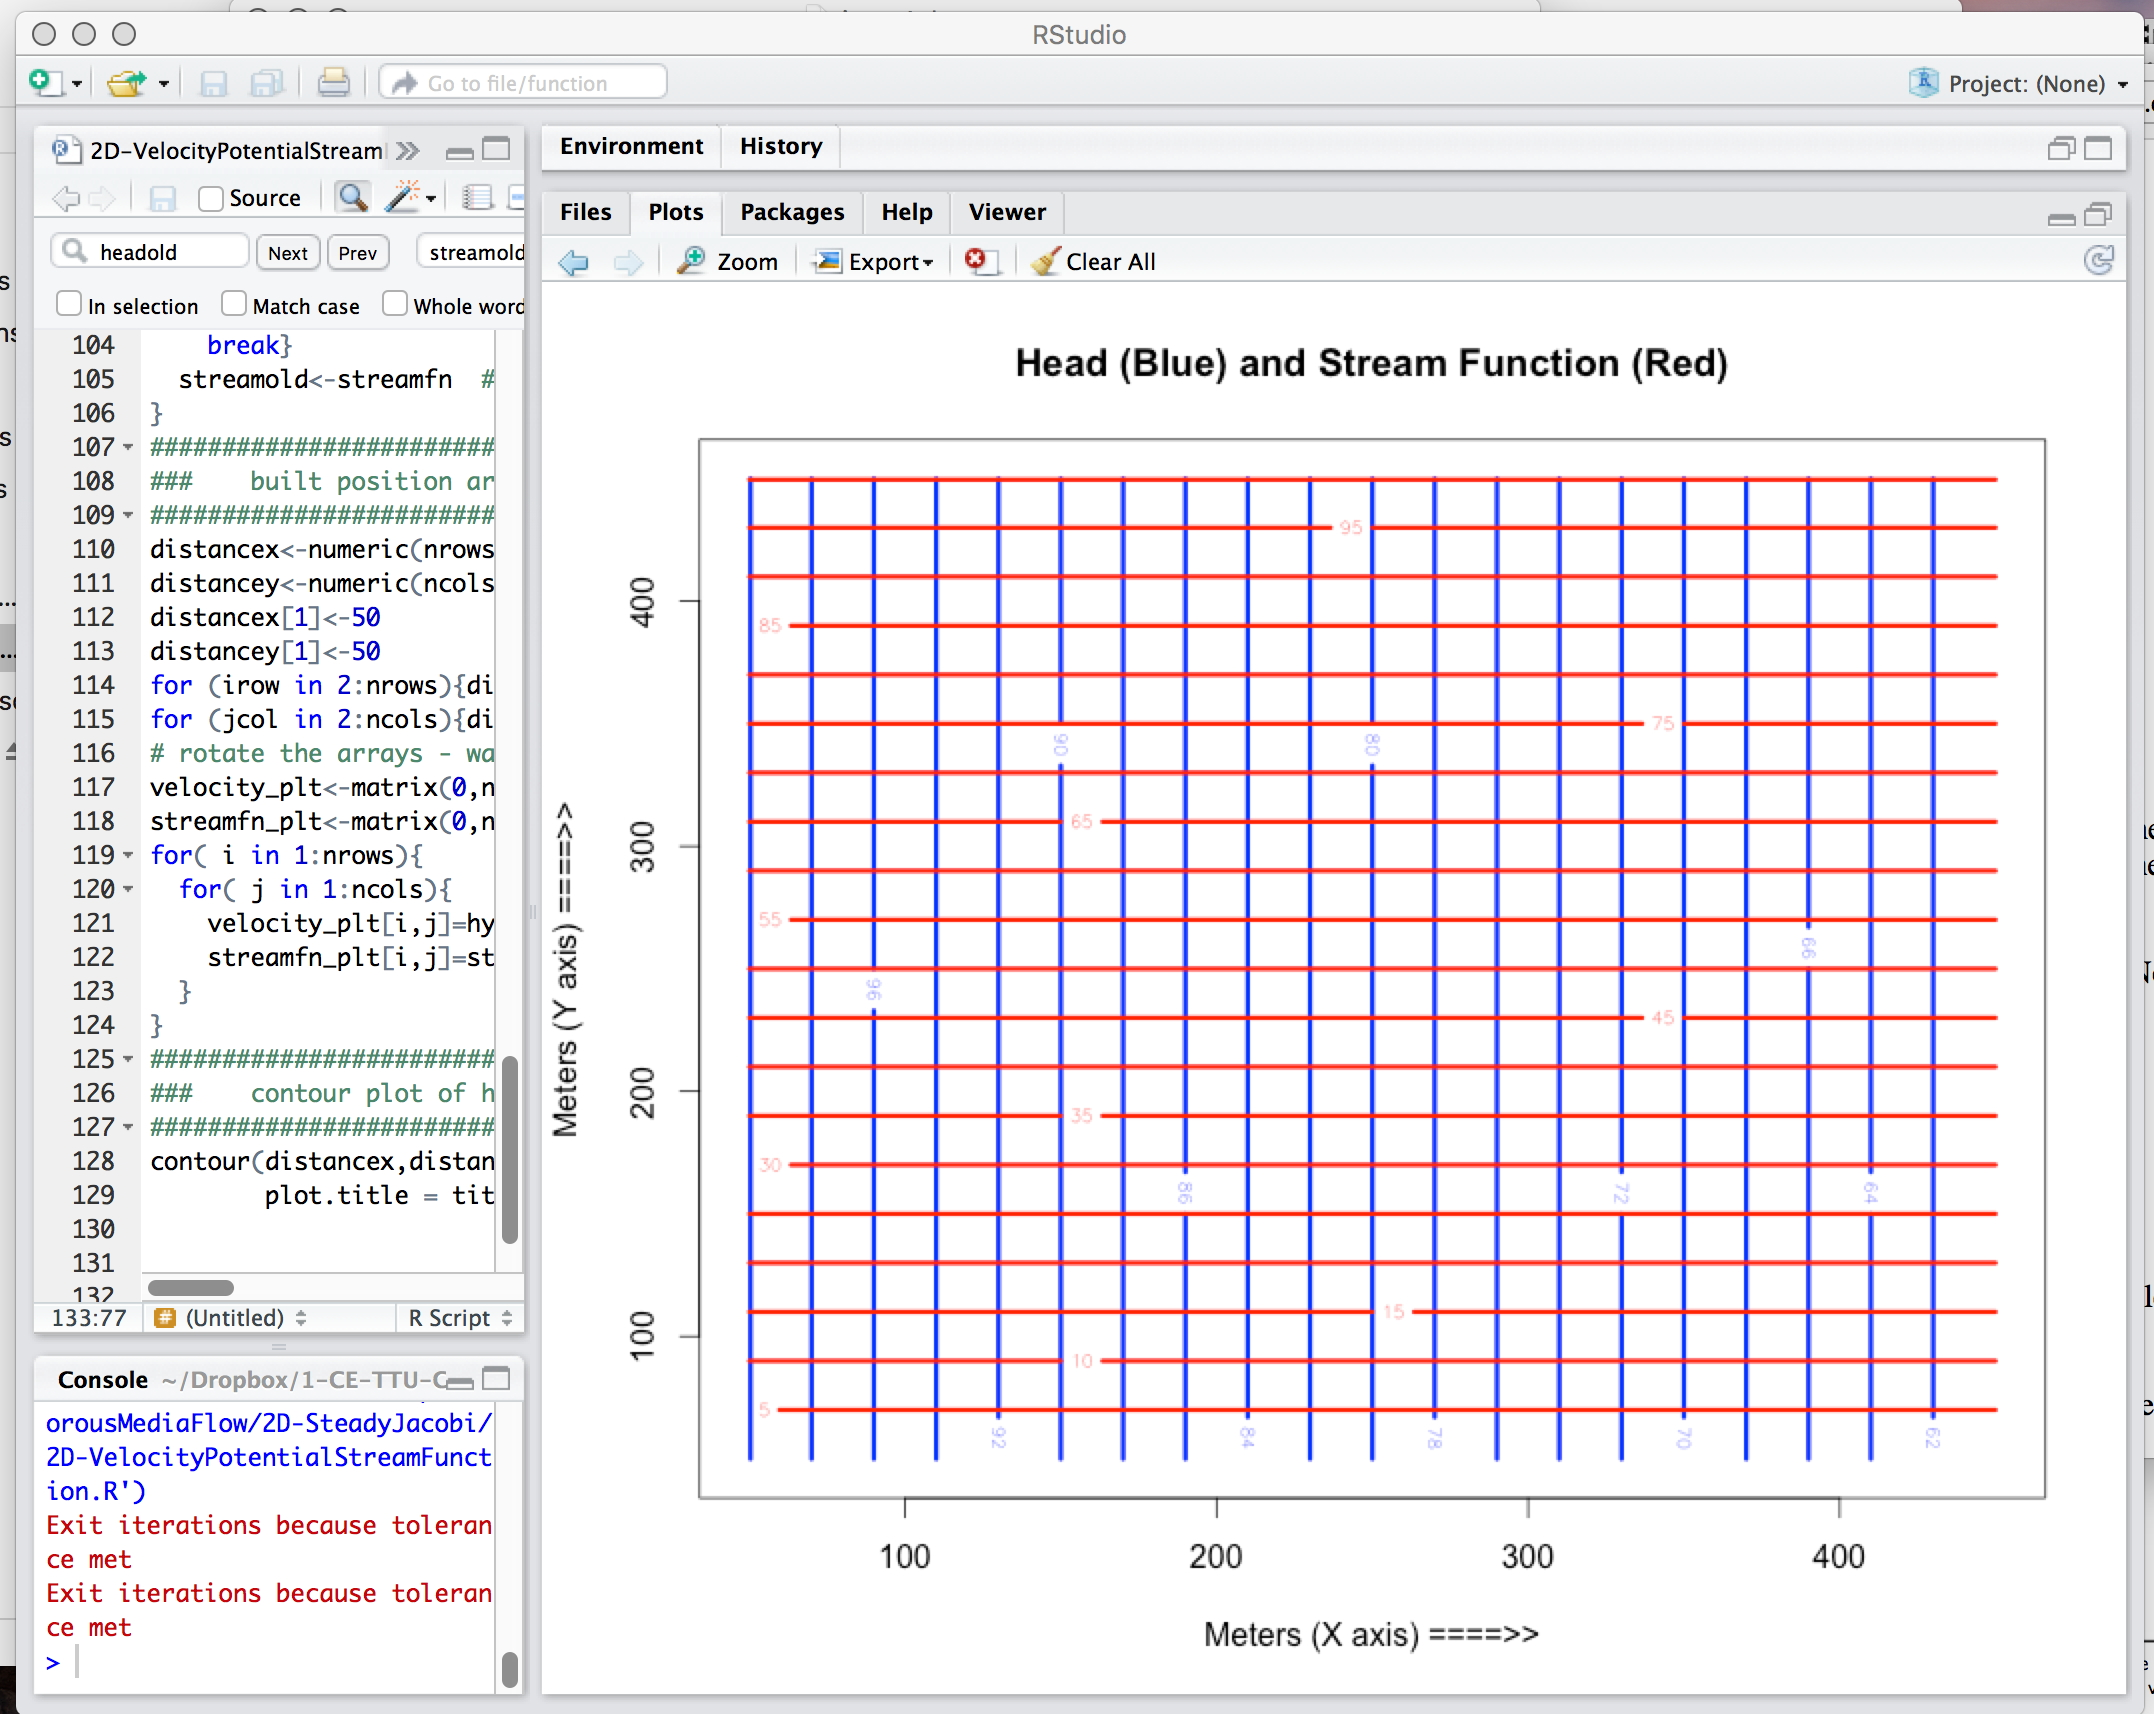
\includegraphics[height=4.5in]{./19-FlowNets/streamfn-2d-contour2.jpg} 
   \caption{Output from \textbf{R} script for velocity-potential, stream function model, rotated and annotated to fit the original problem statement}
   \label{fig:streamfn-2d-contour2}
\end{figure}

Listing \ref{lst:velocitypotential} is a script fragment that implements the velocity-potential (here the same thing as the head equations) portion of the computations.  
The data file is the same, the only difference is the head values are copied to another vector (the stream functions) for use in the next fragment.

Listing \ref{lst:streamfunction} is a script fragment that implements the stream-function calculations.  
The $A,B,C,D$ matrices are re-initialized and re-used.
The stream function values are computed using the same computation engine (code is repeated --  generally poor practice; done here to illustrate the re-use).

Listing \ref{lst:2by2contour} is the script fragment that rotates the results and plots the flow net.
\clearpage

\begin{lstlisting}[caption= R code demonstrating an Velocity Potential (Aquifer Head) Simulator for 2D Steady Flow.  This code fragment implements the contour plotting \\ , label=lst:velocitypotential]
# 2D Velocity Potential Stream Function Model
# hydhead is velocity potential
# streamfm is stream function
zz <- file("input1.dat", "r") # Open a connection named zz to file named input.dat
# read the simulation conditons
deltax <-as.numeric(readLines(zz, n = 1, ok = TRUE, warn = TRUE,encoding = "unknown", skipNul = FALSE))
deltay <-as.numeric(readLines(zz, n = 1, ok = TRUE, warn = TRUE,encoding = "unknown", skipNul = FALSE))
deltaz <-as.numeric(readLines(zz, n = 1, ok = TRUE, warn = TRUE,encoding = "unknown", skipNul = FALSE))
nrows <-as.numeric(readLines(zz, n = 1, ok = TRUE, warn = TRUE,encoding = "unknown", skipNul = FALSE))
ncols <-as.numeric(readLines(zz, n = 1, ok = TRUE, warn = TRUE,encoding = "unknown", skipNul = FALSE))
tolerance <- as.numeric(readLines(zz, n = 1, ok = TRUE, warn = TRUE,encoding = "unknown", skipNul = FALSE))
hydhead <-(readLines(zz, n = nrows, ok = TRUE, warn = TRUE,encoding = "unknown", skipNul = FALSE))
hydcondx <-(readLines(zz, n = nrows, ok = TRUE, warn = TRUE,encoding = "unknown", skipNul = FALSE))
hydcondy <-(readLines(zz, n = nrows, ok = TRUE, warn = TRUE,encoding = "unknown", skipNul = FALSE))
close(zz)
# split the multiple column strings into numeric components for a vector
hydhead <-as.numeric(unlist(strsplit(hydhead,split=" ")))
hydcondx <-as.numeric(unlist(strsplit(hydcondx,split=" ")))
hydcondy <-as.numeric(unlist(strsplit(hydcondy,split=" ")))
# convert the numeric vectors into matrices for easier indexing
hydhead <-matrix(hydhead,nrow=nrows,ncol=ncols,byrow = TRUE)
hydcondx <-matrix(hydcondx,nrow=nrows,ncol=ncols,byrow = TRUE)
hydcondy <-matrix(hydcondy,nrow=nrows,ncol=ncols,byrow = TRUE)
# copy the hydhead array into streamfn for later use
streamfn <- hydhead
# here we perform the velocity potential calculations
# built the transmissivity arrays
amat<-matrix(0,nrows,ncols) 
bmat<-matrix(0,nrows,ncols) 
cmat<-matrix(0,nrows,ncols)
dmat<-matrix(0,nrows,ncols)
for(irow in 2:(nrows-1)){
  for(jcol in 2:(ncols-1)){
    amat[irow,jcol]<-((hydcondx[irow-1,jcol  ]+hydcondx[irow  ,jcol  ])*deltaz)/(2.0*deltax^2)
    bmat[irow,jcol]<-((hydcondx[irow  ,jcol  ]+hydcondx[irow+1,jcol  ])*deltaz)/(2.0*deltax^2)
    cmat[irow,jcol]<-((hydcondy[irow  ,jcol-1]+hydcondy[irow  ,jcol  ])*deltaz)/(2.0*deltay^2)
    dmat[irow,jcol]<-((hydcondy[irow  ,jcol  ]+hydcondy[irow  ,jcol+1])*deltaz)/(2.0*deltay^2)
  }
}
# veloity potential
headold<-hydhead # copy the head array, used to test for stopping 
maxit <- 100 # set the maximum number of iterations (to prevent infinite loop)
for (iter in 1:maxit){
  # first and last row special == no flow boundaries
  for(jcol in 1:ncols){
    hydhead[1,jcol]=hydhead[2,jcol]
    hydhead[nrows,jcol]=hydhead[nrows-1,jcol]
  }
  for (irow in 2:(nrows-1)){
    for (jcol in 2:(nrows-1)){
      hydhead[irow,jcol] = 
        (amat[irow,jcol]*hydhead[irow-1,jcol  ] +
           bmat[irow,jcol]*hydhead[irow+1,jcol  ] +
           cmat[irow,jcol]*hydhead[irow  ,jcol-1] +
           dmat[irow,jcol]*hydhead[irow  ,jcol+1]  )/
        (amat[irow,jcol]+bmat[irow,jcol]+cmat[irow,jcol]+dmat[irow,jcol])
    }
  }
  # test for stopping iterations
  percentdiff <- sum((hydhead-headold)^2)
  if (percentdiff < tolerance){
    message("Exit iterations because tolerance met")
    break}
  headold<-hydhead  #update the current head vector
}
}\end{lstlisting}
\clearpage

\begin{lstlisting}[caption= R code demonstrating an Stream Function Simulator for 2D Steady Flow.  This code fragment implements the stream function \\ , label=lst:streamfunction]
# built the streamfn transmissivity arrays  -- notice reuse of the a,b,c,d arrays
amat<-matrix(0,nrows,ncols) 
bmat<-matrix(0,nrows,ncols) 
cmat<-matrix(0,nrows,ncols)
dmat<-matrix(0,nrows,ncols)
for(irow in 2:(nrows-1)){
  for(jcol in 2:(ncols-1)){
    amat[irow,jcol]<-((1.0/hydcondy[irow-1,jcol  ]+1.0/hydcondy[irow  ,jcol  ])*deltaz)/(2.0*deltax^2)
    bmat[irow,jcol]<-((1.0/hydcondy[irow  ,jcol  ]+1.0/hydcondy[irow+1,jcol  ])*deltaz)/(2.0*deltax^2)
    cmat[irow,jcol]<-((1.0/hydcondx[irow  ,jcol-1]+1.0/hydcondx[irow  ,jcol  ])*deltaz)/(2.0*deltay^2)
    dmat[irow,jcol]<-((1.0/hydcondx[irow  ,jcol  ]+1.0/hydcondx[irow  ,jcol+1])*deltaz)/(2.0*deltay^2)
  }
}
streamold<-streamfn # copy the head array, used to test for stopping 
maxit <- 100 # set the maximum number of iterations (to prevent infinite loop)
for (iter in 1:maxit){
  # first and last row special == no flow boundaries in head, fixed value streamfunction
  for(jcol in 1:ncols){
    streamfn[1,jcol]=0.0
    streamfn[nrows,jcol]=100.0
  }
  for (irow in 2:(nrows-1)){
  # first and last columns special == fixed head boundaries, no-gradient stream function
    streamfn[irow,1]=streamfn[irow,2]
    streamfn[irow,nrows]=streamfn[irow,nrows-1]
    for (jcol in 2:(nrows-1)){
      streamfn[irow,jcol] = 
        (amat[irow,jcol]*streamfn[irow-1,jcol  ] +
         bmat[irow,jcol]*streamfn[irow+1,jcol  ] +
         cmat[irow,jcol]*streamfn[irow  ,jcol-1] +
         dmat[irow,jcol]*streamfn[irow  ,jcol+1]  )/
        (amat[irow,jcol]+bmat[irow,jcol]+cmat[irow,jcol]+dmat[irow,jcol])
    }
  }
# test for stopping iterations
  percentdiff <- sum((streamfn-streamold)^2)
  if (percentdiff < tolerance){
    message("Exit iterations because tolerance met")
    break}
  streamold<-streamfn  #update the current head vector
}
}\end{lstlisting}
\clearpage

\begin{lstlisting}[caption= R code demonstrating an Velocity Potential -- Stream Function Simulator for 2D Steady Flow.  This code fragment implements the contour plotting \\ , label=lst:2by2contour]
##############################################################
###    built position arrays for contour plotting          ###
##############################################################
distancex<-numeric(nrows)
distancey<-numeric(ncols)
distancex[1]<-50
distancey[1]<-50
for (irow in 2:nrows){distancex[irow]<-distancex[irow-1]+deltax}
for (jcol in 2:ncols){distancey[jcol]<-distancey[jcol-1]+deltay}
# rotate the arrays - wasting memory.  Fix for homework.
velocity_plt<-matrix(0,nrows,ncols) 
streamfn_plt<-matrix(0,nrows,ncols) 
for( i in 1:nrows){
  for( j in 1:ncols){
    velocity_plt[i,j]=hydhead[j,i]
    streamfn_plt[i,j]=streamfn[j,i]
  }
}
##############################################################
###    contour plot of head -- note axes are rotated       ###
##############################################################
contour(distancex,distancey,velocity_plt,
        plot.title = title(main = "Head (Blue) and Stream Function (Red)",
                           xlab = "Meters (X axis) ====>>", 
                           ylab = "Meters (Y axis) ====>>"),
        col="blue",lwd=3,xlim=c(50,450),ylim=c(50,450),nlevels=20)
contour(distancey,distancex,streamfn_plt,add=TRUE,col="red",lwd=3,nlevels=20)
}\end{lstlisting}

\clearpage
\textbf{Example 3: 2D Flow Net in a Confined Aquifer using Jacobi Iteration with Low Permeability Inclusion}

Figure \ref{fig:aquifer-2d-lowKinclusion} is a schematic of a different situation that now only requires us to change the contents of the data file, and re-run the scripts unchanged.  
Some additional modifications have been added, mostly messages to the user because of anticipated long run times.    
The data file is changed a bit and two lines are added to help with the plotting -- they represent the axis labels used in the contour plots.
The boundary conditions are still directly coded into the algorithm, and that would be the next modification to the code - general boundary condition information.\footnote{That modification is left for homework.}

\begin{figure}[h!] %  figure placement: here, top, bottom, or page
   \centering
   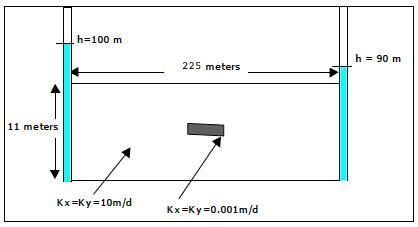
\includegraphics[width=4.5in]{./19-FlowNets/aquifer-2d-lowKinclusion.jpg} 
   \caption{Schematic of vertical slice in an aquifer with low permeability inclusion.  Values are indicated on the schematic.  Example illustrates how to use the scripts to generate flow nets for the vertical slice }
   \label{fig:aquifer-2d-lowKinclusion}
\end{figure}

The following pages contain the code fragments (listings) for the velocity potential, the stream function, and the contour plotting.  As above, these listings are combined into a single file (the fragmentation herein is to fit the printed page layout) and then run as a script. 

Listing \ref{lst:2DinclusionVelocity} is the listing for the velocity potential calculations.

Listing \ref{lst:2DinclusionStream} is the listing for the stream function calculations.

Listing \ref{lst:2DinclusionPlot} is the is the listing for the plotting calculations.

Listing \ref{lst:2DinclusionInput} is the input file for the problem.  The file in this case is named \texttt{input2.dat}.  
In addition the generalized boundary conditons, the reader should consider making the program prompt the user for the file name, so that the program is somewhat deployable.

\clearpage

\begin{lstlisting}[caption= Velocity Potential Script , label=lst:2DinclusionVelocity]
# 2D Velocity Potential Stream Function Model
# hydhead is velocity potential; streamfm is stream function
rm(list=ls())  # deallocate (clear) memory
zz <- file("input2.dat", "r") # Open a connection named zz to file named input.dat to read input conditions
deltax <-as.numeric(readLines(zz, n = 1, ok = TRUE, warn = TRUE,encoding = "unknown", skipNul = FALSE))
deltay <-as.numeric(readLines(zz, n = 1, ok = TRUE, warn = TRUE,encoding = "unknown", skipNul = FALSE))
deltaz <-as.numeric(readLines(zz, n = 1, ok = TRUE, warn = TRUE,encoding = "unknown", skipNul = FALSE))
nrows <-as.numeric(readLines(zz, n = 1, ok = TRUE, warn = TRUE,encoding = "unknown", skipNul = FALSE))
ncols <-as.numeric(readLines(zz, n = 1, ok = TRUE, warn = TRUE,encoding = "unknown", skipNul = FALSE))
tolerance <- as.numeric(readLines(zz, n = 1, ok = TRUE, warn = TRUE,encoding = "unknown", skipNul = FALSE))
distancex <- (readLines(zz, n = 1, ok = TRUE, warn = TRUE,encoding = "unknown", skipNul = FALSE))
distancey <- (readLines(zz, n = 1, ok = TRUE, warn = TRUE,encoding = "unknown", skipNul = FALSE))
hydhead <-(readLines(zz, n = nrows, ok = TRUE, warn = TRUE,encoding = "unknown", skipNul = FALSE))
hydcondx <-(readLines(zz, n = nrows, ok = TRUE, warn = TRUE,encoding = "unknown", skipNul = FALSE))
hydcondy <-(readLines(zz, n = nrows, ok = TRUE, warn = TRUE,encoding = "unknown", skipNul = FALSE))
close(zz)
# split the multiple column strings into numeric components for a vector
distancex <-as.numeric(unlist(strsplit(distancex,split=" ")))
distancey <-as.numeric(unlist(strsplit(distancey,split=" ")))
hydhead <-as.numeric(unlist(strsplit(hydhead,split=" ")))
hydcondx <-as.numeric(unlist(strsplit(hydcondx,split=" ")))
hydcondy <-as.numeric(unlist(strsplit(hydcondy,split=" ")))
# convert the numeric vectors into matrices for easier indexing
hydhead <-matrix(hydhead,nrow=nrows,ncol=ncols,byrow = TRUE)
hydcondx <-matrix(hydcondx,nrow=nrows,ncol=ncols,byrow = TRUE)
hydcondy <-matrix(hydcondy,nrow=nrows,ncol=ncols,byrow = TRUE)
# built the transmissivity arrays
amat<-matrix(0,nrows,ncols) 
bmat<-matrix(0,nrows,ncols) 
cmat<-matrix(0,nrows,ncols)
dmat<-matrix(0,nrows,ncols)
for(irow in 2:(nrows-1)){
  for(jcol in 2:(ncols-1)){
    amat[irow,jcol]<-((hydcondx[irow-1,jcol  ]+hydcondx[irow  ,jcol  ])*deltaz)/(2.0*deltax^2)
    bmat[irow,jcol]<-((hydcondx[irow  ,jcol  ]+hydcondx[irow+1,jcol  ])*deltaz)/(2.0*deltax^2)
    cmat[irow,jcol]<-((hydcondy[irow  ,jcol-1]+hydcondy[irow  ,jcol  ])*deltaz)/(2.0*deltay^2)
    dmat[irow,jcol]<-((hydcondy[irow  ,jcol  ]+hydcondy[irow  ,jcol+1])*deltaz)/(2.0*deltay^2)
  }
}
headold<-hydhead      # copy the head array, used to test for stopping 
tolflag<-FALSE
maxit <- 500000 # set the maximum number of iterations (to prevent infinite loop)
for (iter in 1:maxit){
  # first and last row special == no flow boundaries
  for(jcol in 1:ncols){
    hydhead[1,jcol]<-hydhead[2,jcol]
    hydhead[nrows,jcol]<-hydhead[nrows-1,jcol]
  }
  for (irow in 2:(nrows-1)){
    for (jcol in 2:(ncols-1)){
      hydhead[irow,jcol] <- 
        (amat[irow,jcol]*hydhead[irow-1,jcol  ] +
           bmat[irow,jcol]*hydhead[irow+1,jcol  ] +
           cmat[irow,jcol]*hydhead[irow  ,jcol-1] +
           dmat[irow,jcol]*hydhead[irow  ,jcol+1]  )/
        (amat[irow,jcol]+bmat[irow,jcol]+cmat[irow,jcol]+dmat[irow,jcol])
    }
  }
  # test for stopping iterations
  percentdiff <- sum((hydhead-headold)^2)
  if (percentdiff < tolerance){
    message("Exit iterations in velocity potential because tolerance met");
    message("Iterations =", iter);
    tolflag <- TRUE
    break}
 headold<-hydhead  #update the current head vector
 if( iter %% 5000 == 0){message("Calculating in Potential Function ",iter," of ",maxit, "iterations")}
}
if (tolflag == FALSE){message("Exit iterations in potential function at max iterations")}
}\end{lstlisting}








\begin{lstlisting}[caption= Stream Function Script , label=lst:2DinclusionStream]
streamfn<-matrix(1.0,nrows,ncols)
for (i in 1:nrows){
  for(j in 1:ncols){
    streamfn[i,j]=as.numeric(i)/as.numeric(nrows)
  }
}
streamfn
# built the streamfn transmissivity arrays
amats<-matrix(0,nrows,ncols) 
bmats<-matrix(0,nrows,ncols) 
cmats<-matrix(0,nrows,ncols)
dmats<-matrix(0,nrows,ncols)
for(irow in 2:(nrows-1)){
  for(jcol in 2:(ncols-1)){
    amats[irow,jcol]<-((1.0/hydcondy[irow-1,jcol  ]+1.0/hydcondy[irow  ,jcol  ])*deltaz)/(2.0*deltax^2)
    bmats[irow,jcol]<-((1.0/hydcondy[irow  ,jcol  ]+1.0/hydcondy[irow+1,jcol  ])*deltaz)/(2.0*deltax^2)
    cmats[irow,jcol]<-((1.0/hydcondx[irow  ,jcol-1]+1.0/hydcondx[irow  ,jcol  ])*deltaz)/(2.0*deltay^2)
    dmats[irow,jcol]<-((1.0/hydcondx[irow  ,jcol  ]+1.0/hydcondx[irow  ,jcol+1])*deltaz)/(2.0*deltay^2)
  }
}
streamold<-streamfn # copy the head array, used to test for stopping 
tolflag<-FALSE
maxit <- maxit/10 # set the maximum number of iterations (to prevent infinite loop)
for (iter in 1:maxit){
  # first and last row special == no flow boundaries in head, fixed value streamfunction
  for(jcol in 1:ncols){
    streamfn[1,jcol]=0.0
    streamfn[nrows,jcol]=1.0
  }
  for (irow in 2:(nrows-1)){
    # first and last columns special == fixed head boundaries, no-gradient stream function
    streamfn[irow,1]=streamfn[irow,2]
    streamfn[irow,ncols]=streamfn[irow,ncols-1]
    for (jcol in 2:(ncols-1)){
      streamfn[irow,jcol] = 
        (amats[irow,jcol]*streamfn[irow-1,jcol  ] +
           bmats[irow,jcol]*streamfn[irow+1,jcol  ] +
           cmats[irow,jcol]*streamfn[irow  ,jcol-1] +
           dmats[irow,jcol]*streamfn[irow  ,jcol+1]  )/
        (amats[irow,jcol]+bmats[irow,jcol]+cmats[irow,jcol]+dmats[irow,jcol])
    }
  }
  # test for stopping iterations
  percentdiff <- sum((streamfn-streamold)^2)
  if (percentdiff < tolerance)
    {
    message("Exit iterations in stream function because tolerance met");
    message("Iterations =", iter);
    tolflag <- TRUE;
    break
    }
  streamold<-streamfn  #update the current head vector
  if( iter %% 5000 == 0){message("Calculating in Stream Function ",iter," of ",maxit, "iterations")}
}
if (tolflag == FALSE){message("Exit iterations in stream function at max iterations")}
}\end{lstlisting}















\begin{lstlisting}[caption= Contour plotting script , label=lst:2DinclusionPlot]
###############################################################################
###    rotate arrays for contour plotting -- position values read in input  ###
###############################################################################
velocity_plt<-matrix(0,ncols,nrows) 
streamfn_plt<-matrix(0,ncols,nrows) 
for( i in 1:nrows){
  for( j in 1:ncols){
    velocity_plt[j,i]=hydhead[i,j]
    streamfn_plt[j,i]=streamfn[i,j]
  }
}
##############################################################
###    contour plot of head -- note axes are rotated       ###
##############################################################
contour(distancey,distancex,velocity_plt,
        plot.title = title(main = "Head (Blue) and Stream Function (Red)",
                           xlab = "Meters (X axis) ====>>", 
                           ylab = "Meters (Y axis) ====>>"),
        col="blue",lwd=3,nlevels=20)
contour(distancey,distancex,streamfn_plt,add=TRUE,col="red",lwd=3,nlevels=20)
}\end{lstlisting}

\begin{lstlisting}[caption= Input file for 2D vertical slice confined aquifer with low permeability inclusion , label=lst:2DinclusionInput]
1
10
1
13
23
1e-16
0.5 1.5 2.5 3.5 4.5 5.5 6.5 7.5 8.5 9.5 10.5 11.5 12.5
5 15 25 35 45 55 65 75 85 95 105 115 125 135 145 155 165 175 185 195 205 215 225
100 100 100 100 100 100 100 100 100 100 100 100 100 100 100 100 100 100 100 100 100 100 90
100 100 100 100 100 100 100 100 100 100 100 100 100 100 100 100 100 100 100 100 100 100 90
100 100 100 100 100 100 100 100 100 100 100 100 100 100 100 100 100 100 100 100 100 100 90
100 100 100 100 100 100 100 100 100 100 100 100 100 100 100 100 100 100 100 100 100 100 90
100 100 100 100 100 100 100 100 100 100 100 100 100 100 100 100 100 100 100 100 100 100 90
100 100 100 100 100 100 100 100 100 100 100 100 100 100 100 100 100 100 100 100 100 100 90
100 100 100 100 100 100 100 100 100 100 100 100 100 100 100 100 100 100 100 100 100 100 90
100 100 100 100 100 100 100 100 100 100 100 100 100 100 100 100 100 100 100 100 100 100 90
100 100 100 100 100 100 100 100 100 100 100 100 100 100 100 100 100 100 100 100 100 100 90
100 100 100 100 100 100 100 100 100 100 100 100 100 100 100 100 100 100 100 100 100 100 90
100 100 100 100 100 100 100 100 100 100 100 100 100 100 100 100 100 100 100 100 100 100 90
100 100 100 100 100 100 100 100 100 100 100 100 100 100 100 100 100 100 100 100 100 100 90
100 100 100 100 100 100 100 100 100 100 100 100 100 100 100 100 100 100 100 100 100 100 90
10 10 10 10 10 10 10 10 10 10 10 10 10 10 10 10 10 10 10 10 10 10 10
10 10 10 10 10 10 10 10 10 10 10 10 10 10 10 10 10 10 10 10 10 10 10
10 10 10 10 10 10 10 10 10 10 10 10 10 10 10 10 10 10 10 10 10 10 10
10 10 10 10 10 10 10 10 10 10 10 10 10 10 10 10 10 10 10 10 10 10 10
10 10 10 10 10 10 10 10 10 10 10 10 10 10 10 10 10 10 10 10 10 10 10
10 10 10 10 10 10 10 10 10 10 0.0001 0.0001 0.0001 10 10 10 10 10 10 10 10 10 10
10 10 10 10 10 10 10 10 10 10 0.0001 0.0001 0.0001 10 10 10 10 10 10 10 10 10 10
10 10 10 10 10 10 10 10 10 10 0.0001 0.0001 0.0001 10 10 10 10 10 10 10 10 10 10
10 10 10 10 10 10 10 10 10 10 10 10 10 10 10 10 10 10 10 10 10 10 10
10 10 10 10 10 10 10 10 10 10 10 10 10 10 10 10 10 10 10 10 10 10 10
10 10 10 10 10 10 10 10 10 10 10 10 10 10 10 10 10 10 10 10 10 10 10
10 10 10 10 10 10 10 10 10 10 10 10 10 10 10 10 10 10 10 10 10 10 10
10 10 10 10 10 10 10 10 10 10 10 10 10 10 10 10 10 10 10 10 10 10 10
10 10 10 10 10 10 10 10 10 10 10 10 10 10 10 10 10 10 10 10 10 10 10
10 10 10 10 10 10 10 10 10 10 10 10 10 10 10 10 10 10 10 10 10 10 10
10 10 10 10 10 10 10 10 10 10 10 10 10 10 10 10 10 10 10 10 10 10 10
10 10 10 10 10 10 10 10 10 10 10 10 10 10 10 10 10 10 10 10 10 10 10
10 10 10 10 10 10 10 10 10 10 10 10 10 10 10 10 10 10 10 10 10 10 10
10 10 10 10 10 10 10 10 10 10 0.0001 0.0001 0.0001 10 10 10 10 10 10 10 10 10 10
10 10 10 10 10 10 10 10 10 10 0.0001 0.0001 0.0001 10 10 10 10 10 10 10 10 10 10
10 10 10 10 10 10 10 10 10 10 0.0001 0.0001 0.0001 10 10 10 10 10 10 10 10 10 10
10 10 10 10 10 10 10 10 10 10 10 10 10 10 10 10 10 10 10 10 10 10 10
10 10 10 10 10 10 10 10 10 10 10 10 10 10 10 10 10 10 10 10 10 10 10
10 10 10 10 10 10 10 10 10 10 10 10 10 10 10 10 10 10 10 10 10 10 10
10 10 10 10 10 10 10 10 10 10 10 10 10 10 10 10 10 10 10 10 10 10 10
10 10 10 10 10 10 10 10 10 10 10 10 10 10 10 10 10 10 10 10 10 10 10
}\end{lstlisting}

Lastly, the result of running the script on the input file is shown in figure \ref{fig:LowPInclusionOut}

\begin{figure}[h!] %  figure placement: here, top, bottom, or page
   \centering
   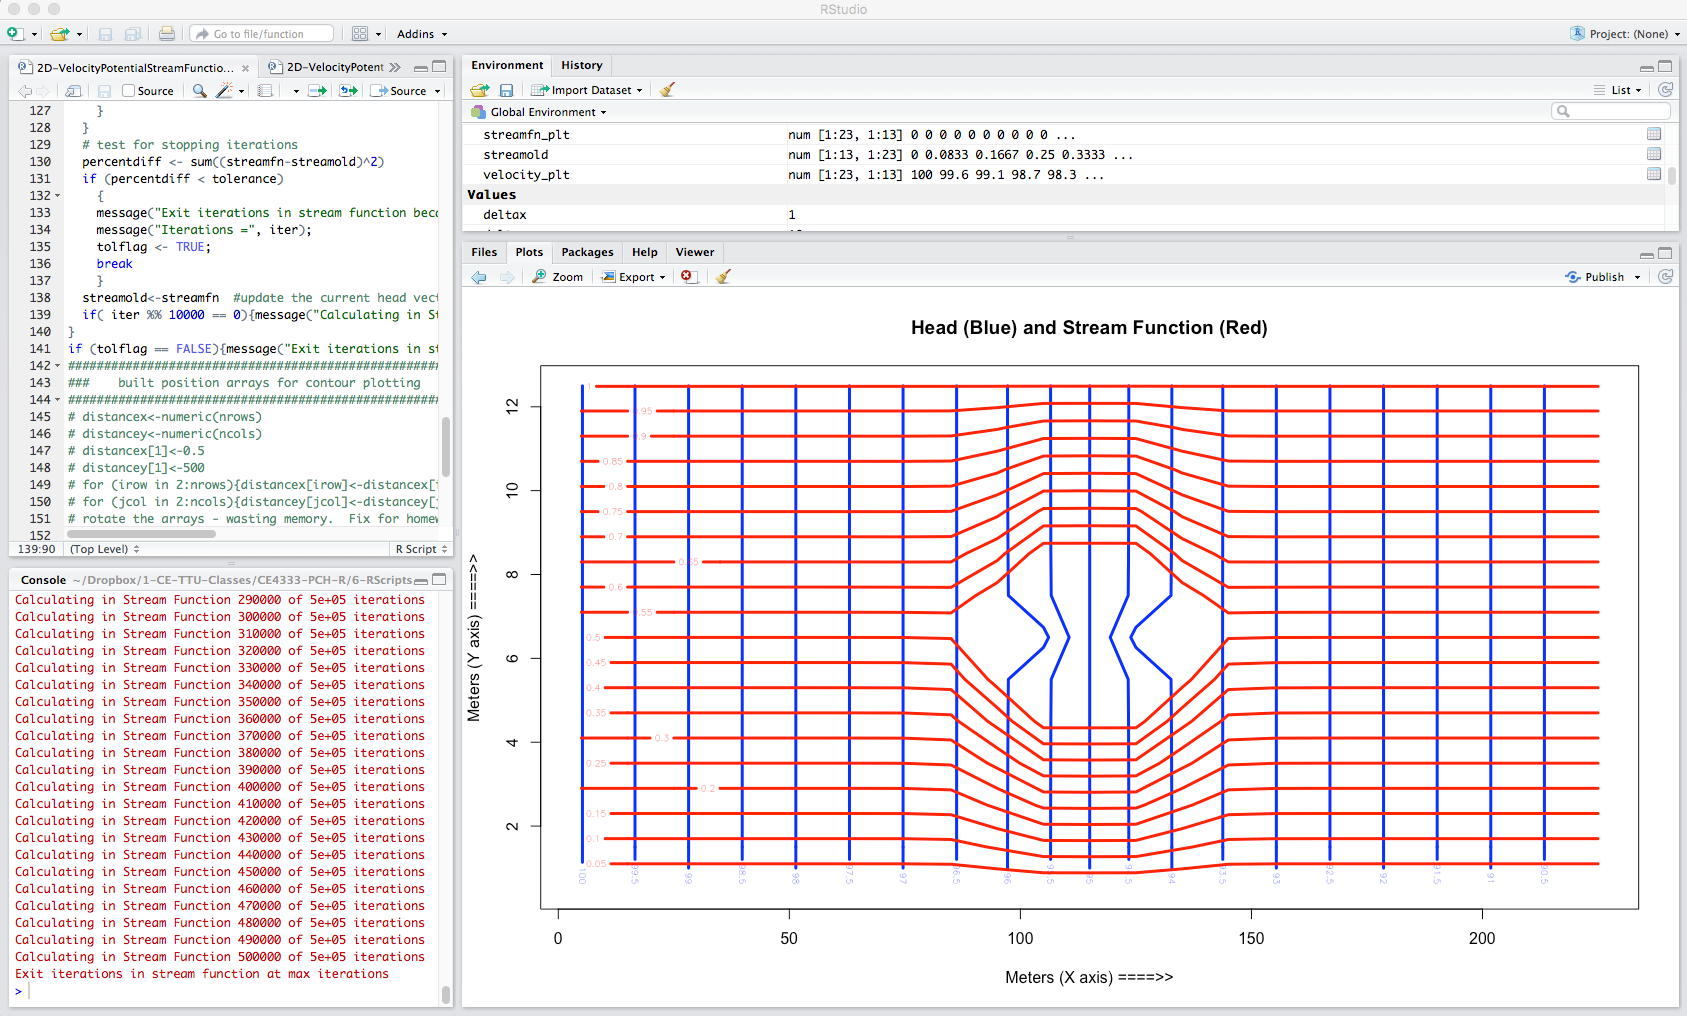
\includegraphics[width=5.2in]{./19-FlowNets/LowPInclusionOut.jpg} 
   \caption{Vertical slice in an aquifer with low permeability inclusion using Jacobi iteration scripts}
   \label{fig:LowPInclusionOut}
\end{figure}

[Modifications to handle generalized boundary conditions]



\clearpage
\subsection{Unconfined Aquifer Flow}
\subsubsection{Finite-Difference Methods}
\subsection{Exercises}